\section{Этап Render pass} \label{ch3:render_pass}
	\begin{figure}[ht!] 
		\center
		
\includegraphics [scale=0.4] {my_folder/images//renderpass_schema}	
		\caption{Схема этапа Render pass предлагаемого конвеера.} 
		\label{fig:renderpass_schema}
	\end{figure}
	
	На данном этапе, после всей подготовительной работы, поведённой в предыдущем этапе, происходит отрисовка объектов на кадр.
	
	\subsection{Непрозрачные объекты} \label{ch3:render_pass:opaque}
		Данный подэтап отвечает за отрисовку всех непрозрачных объектов, используя буфер OpaqueCulled, карту глубины из главы \ref{ch3:pre_pass:depth} и карты теней из главы \ref{ch3:pre_pass:shadow_maps}.
		
		Для отображения объектов с учётом их материала и расположения относительно источников света используются различные модели освещения. В предлагаемой архитектуре используется алгоритм модели освещения, называющийся Physically based rendering.
	
		\subsubsection{Physically based rendering} \label{ch3:render_pass:opaque:pbr}
			Данный алгоритм освещения использует в своей основе физическую модель микрограней. В этой физической модели поверхность любого объекта представляют собой множество идеальных зеркал, находящихся под разными углами друг к другу (см \firef{fig:microfacet}).
			
			\begin{figure}[ht!] 
				\center
				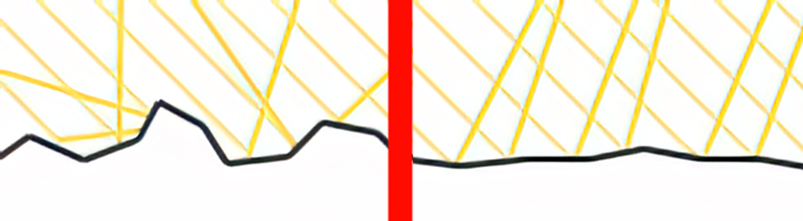
\includegraphics [scale=0.4] {my_folder/images//microfacet}	
				\caption{Схема физической модели микрограней. Слева - шершавая поверхность, справа - гладкая} 
				\label{fig:microfacet}
			\end{figure}
			
			Для понимания принципов работы алгоритма Physically based rendering необходимо рассмотреть \say{Основное уравнение рендеринга} \ref{eq:rendering}, предложенное Джеймсом Каджия. 
			
			\begin{equation}
				\label{eq:rendering}
				\begin{multlined}
					L_o(x, \omega_o) = L_e(x, \omega_o) + \int_{\Omega} f_r(x, \omega_i, \omega_o)L_i(x, \omega_i)(n_x * \omega_i)d\omega_i
				\end{multlined}
			\end{equation}
			
			Данное уравнение показывает, что интенсивность света в точке $x$ по направлению $\omega_o$ равна сумме излучемой интенсивности($L_e(x, \omega_o)$) и отраженной интенсивности, где последняя считается как интеграл по полусфере произведения интенсивности падающего света ($L_i(x, \omega_i)$), двунаправленной функции отражательной способности($f_r(x, \omega_i, \omega_o)$) и косинуса угла падения($(n_x * \omega_i)$). Двунаправленая функция отражательной способности $f_r$ часто называется BRDF функцией. 
			
			\begin{figure}[ht!] 
				\center
				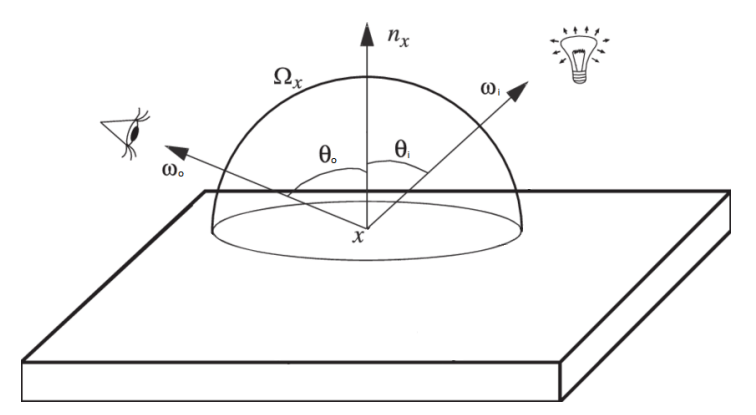
\includegraphics [scale=0.6] {my_folder/images//rendering_eq}	
				\caption{Обозначения используемые в "основном уравнении рендеринга"} 
				\label{fig:base_rendering}
			\end{figure}
			
			В предлагаемом конвейере используется BRDF функция Кука-Торренса.
		%TODO: \subsubsection{Image based lighting} \label{ch3:render_pass:opaque:ibl}
	\subsection{Skybox} \label{ch3:render_pass:skybox}
		На данном подэтапе в кадр выводится фоновое изображение, на котором изображено окружение сцены. Данный подэтап рисуется после отрисовки непрозрачных объектов, чтобы уменьшить число перерисовываемых пикселей кадра, так как фоновое изображение рисуется только в тех пикселях, не не были отрисованы объекты. 
		
		Описанное фоновое изображение представляется как 6 изображений, снятых с 6-ти направлений и расположенных в развёртке куба, как показано на \firef{fig:skybox}.
		
		\begin{figure}[ht!] 
			\center
			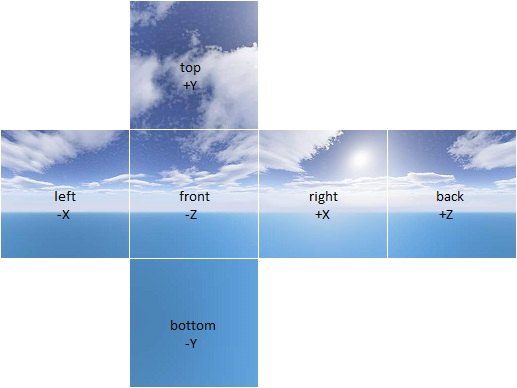
\includegraphics [scale=0.4] {my_folder/images//skybox}	
			\caption{Развётка фонового изображения} 
			\label{fig:skybox}
		\end{figure}
		
		Таким образом, при необходимости вывести цвет в пикселе, в котором не были отрисованы объекты, достаточно будет посчитать направление, к котором этот пиксель находится, и взять точку, соответствующую точке на кубе, в указаном направлении(см. \firef{fig:cube_sample}).
		
		\begin{figure}[ht!] 
			\center
			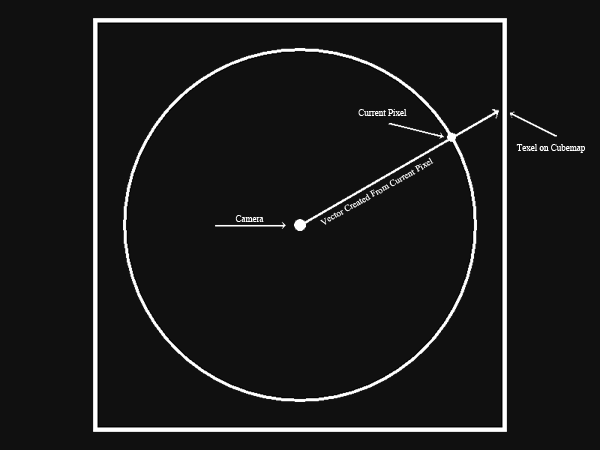
\includegraphics [scale=0.4] {my_folder/images//cube_sample}	
			\caption{Схема работы вычисления цвета пикселя используя кубическую развертку} 
			\label{fig:cube_sample}
		\end{figure}
		
	\subsection{Полу-прозрачные объекты} \label{ch3:render_pass:transparents}
		На данном подэтапе в кадр выводятся полупрозрачные объекты при помощи буфера TransparentCulled. Как понятно из названия, полу-прозрачные объекты отличаются от непрозрачных тем, что через них можно видеть объекты находящиеся позади. Из-за этого, нельзя воспользоваться картой глубины(cм. главу \ref{ch3:pre_pass:depth}) для отрисовки только ближайшего пикселя, что может привести к ситуации, приведённой на \firef{fig:incorrect_transparent}.
		
		\begin{figure}[ht!] 
			\center
			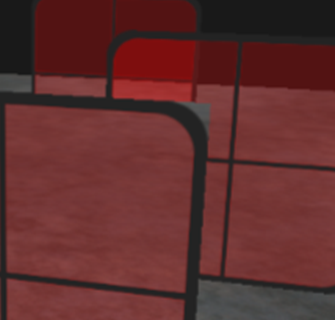
\includegraphics [scale=0.5] {my_folder/images//incorrect_transparent}	
			\caption{Пример отрисовки прозрачных объектов в неправильном порядке} 
			\label{fig:incorrect_transparent}
		\end{figure}
		\FloatBarrier
		
		Чтобы избежать изображенной ситуации, необходимо производить сортировку объектов. Тогда, если выводить объекты начиная с самого дальнего, то цвет в пикселе можно вычислять по формуле \ref{eq:blend-formula}.
		
		\begin{equation}
			\label{eq:blend-formula}
			\begin{multlined}
				C_{new} = \alpha * C_{transparent} + (1 - \alpha) * C_{pixel}
			\end{multlined}
		\end{equation}
		
		Где:
		\begin{enumerate}[1.]
			\item $C_{new}$ - новый цвет пиксела
			\item $C_{transparent}$ - цвет полученный в результате применения алгоритма освещения, для данного пиксела
			\item $C_{pixel}$ - цвет, хранящийся в данном пикселе.
			\item $\alpha$ - коэффициент прозрачности. Значение 0 обозначает абсолютно прозрачный объект, значение 1 абсолютно непрозрачный объект.
		\end{enumerate}
		
		Однако предлагаемый алгоритм неявной отрисовки(см главу \ref{ch3:indirect_draw}) не позволяет установить порядок отрисовки объектов. Из-за этого необходимо использовать особые алогритмы отрисовки прозрачных объектов.		
		
		\subsubsection{Order Independent Transparency} \label{ch3:render_pass:transparents:oit}
			Первым из рассмотренных алгоритмов является алгоритм Order Independent Transparency with per-pixel linked lists \cite{barta2011order}. В данном алгоритме, для каждого пиксела экрана заводится список, в каждом элементе которого хранится: цвет, глубина и коэффициент прозрачности. Далее алгоритм работает в 2 запуска отрисовки
			
			\begin{enumerate}[1.]
				\item Отрисовываются все полупрозрачные объекты, но результат отрисовки объекта записывается не в кадр, а добавляется в конец созданных списков.
				\item На экран отрисовывается прямоугольник, покрывающий весь экран. Для каждого пиксела прямоугольника берётся соответсвующий ему список и значения в этом списке сортируются по глубине. Далее, используя отсортированный список, последовательно применим формулу \ref{eq:blend-formula} и получим формулу для итогового цвета \ref{eq:oit-formula}.
			\end{enumerate}
			
			\begin{figure}[ht!] 
				\center
				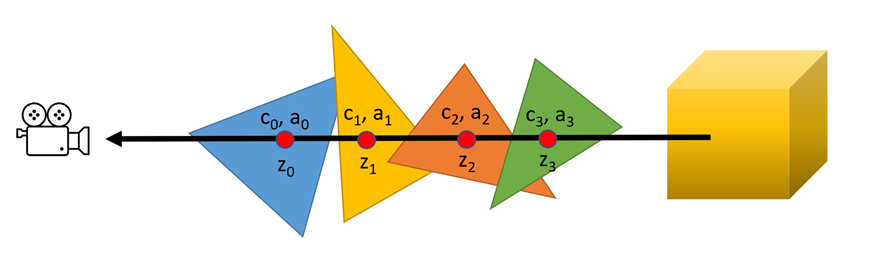
\includegraphics [scale=0.5] {my_folder/images//first_step_oit}	
				\caption{Изображение демонстрирующее первый этап работы алгоритма} 
				\label{fig:first_step_oit}
			\end{figure}
			 
			\begin{equation}
				\label{eq:oit-formula}
				\begin{multlined}	 
			 		C_{out} = C_{1}\alpha_1 + \sum_{i=2}^{N}(C_i\alpha_i\prod _{j=1}^{i - 1}(1 - \alpha_j)) + 
			 		C_{opaque}\prod _{j=1}^{N}(1 - \alpha_j)   
			 	\end{multlined}
			 \end{equation}
			
			Где:
			\begin{enumerate}[1.]
				\item $N$ - размер списка для данного пиксела
				\item $C_{out}$ - результирующий цвет пиксела
				\item $C_{opaque}$ - цвет непрозрачного объекта, полученный из пиксела кадра.
				\item $C_{i}$ - цвет, полученный из элемента отсортированного списка с номером $i$.
				\item $\alpha_i$ - коэффициент прозрачности, полученный из элемента отсортированного списка с номером $i$.
			\end{enumerate}			
			
			Нетрудно заметить, что благодаря переносу сортировки на второй этап, появляется возможность отрисовывать объекты на первом этапе в любом порядке. Однако время, требуемое на выполнение вышеописанной сортировки, сильно сказывается на производительности. Авторами статьи упоминается, что количество отрисовываемых кадров в секунду при использовании данного подхода, падает с 110 вплоть до 5. Это означает, что запуск отрисовки с сортировкой может занимать до 190 миллисекунд.			
		\subsubsection{Weighted Blended Order Independent Transparency} \label{ch3:render_pass:transparents:wboit}
			В 2013 году, в качестве улучшения предыдущего алгоритма, был представлен алгоритм Weighted Blended Order Independent Transparency\cite{mcguire2013weighted}. Данный алгоритм повторяет идею предыдущего алгоритма, однако вместо сортировки и применения формулы \ref{eq:oit-formula}, предлагается использовать её аппроксимацию \ref{eq:wboit-formula}
					 
			\begin{equation}
				\label{eq:wboit-formula}
				\begin{multlined}	 
					C_{out} = \frac{\sum_{i=1}^{N}C_i}{\sum_{i=1}^{N}\alpha_i}(1 - \prod_{i=1}^{N}\alpha_i) + 
					C_{opaque}\prod _{j=1}^{N}(1 - \alpha_j)   
				\end{multlined}
			\end{equation}
			
			Очевидно, что данная аппроксимация работает гораздо быстрее подхода описаного в оригинальном алгоритме. Однако, при коэффициентах $\alpha_i$ близких к 1-це, погрешности аппроксимации становятся явно заметны человеческому глазу. Визуальное сравнение можно увидеть на \firef{fig:oit_vs_wboit}.
			
			\begin{figure}[!htbp]
				\centering
				\begin{subfigure}[b]{0.3\textwidth}
					\centering
					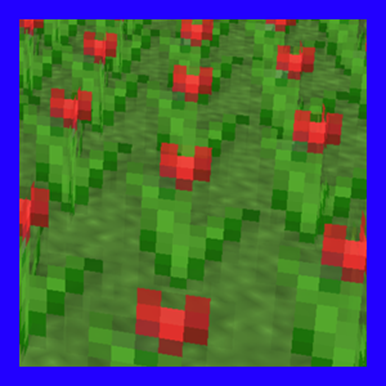
\includegraphics[width=\textwidth]{my_folder/images//oit_flower}
					\caption{Изображение полученное алгоритмом OIT.\linebreak Время построения кадра: 6.2ms}
					\label{fig:oit_flower}
				\end{subfigure}
				\begin{subfigure}[b]{0.3\textwidth}
					\centering
					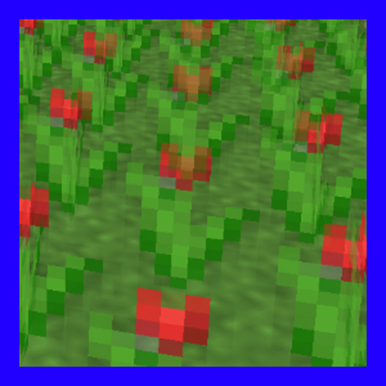
\includegraphics[width=\textwidth]{my_folder/images//wboit_flower}
					\caption{Изображение полученное алгоритмом WBOIT.\linebreak Время построения кадра: 1.9ms}
					\label{fig:wboit_flower}
				\end{subfigure}				
				\captionsetup{justification=centering} %центрировать
				\caption{Сравнение работы алгоритмов OIT и WBOIT}\label{fig:oit_vs_wboit} 
			\end{figure}
			
		\subsubsection{Hybrid Order Independent Transparency} \label{ch3:render_pass:transparents:hybrid_oit}
			В результате изучения описаных алгоритмов, было решено разработать новый, гибридный алгоритм, совмещающий в себе преимущества описанных алгоритмов. Как и предыдущие алгоритмы, он состоит из двух запусков отрисовки:
			
			\begin{enumerate}[1.]
				\item Как и в предыдущих алгоритмах, все полупрозрачные объекты отрисовываются в списки, созданные для каждого пиксела.
				\item В списках для каждого пикслела, вместо сортировки всего списка, находятся $K$ наименьших по параметру глубины, и они сортируются между собой. Затем результирующий цвет вычисляется по формуле \ref{eq:hybrid-formula}
			\end{enumerate}
			
			\begin{equation}
				\label{eq:oit-formula}
				\begin{multlined}	 
					C_{out} = C_{1}\alpha_1 +
					\sum_{i=2}^{K}(C_i\alpha_i\prod _{j=1}^{i - 1}(1 - \alpha_j)) + \\
					\frac{\sum_{i=K+1}^{N}C_i}{\sum_{i=K+1}^{N}\alpha_i}(1 - \prod_{i=K+1}^{N}\alpha_i)\prod _{i=1}^{K}(1 - \alpha_i) + \\	
					C_{opaque}\prod _{j=1}^{N}(1 - \alpha_j)   
				\end{multlined}
			\end{equation}
			
			Как можно заметить, данный алгоритм смешивает $N-K$ элементов списка по формуле \ref{eq:wboit-formula}, а затем, считая получившийся цвет, как элемент списка с номером $K+1$, применяет формулу \ref{eq:oit-formula}, считая что список состоит из $K+1$ элемента. Визуальное сравнение всех трех методов можно увидеть на \firef{fig:oit_vs_wboit_vs_hybrid}.
		
			\begin{figure}[!htbp]
				\centering
				\begin{subfigure}[b]{0.3\textwidth}
					\centering
					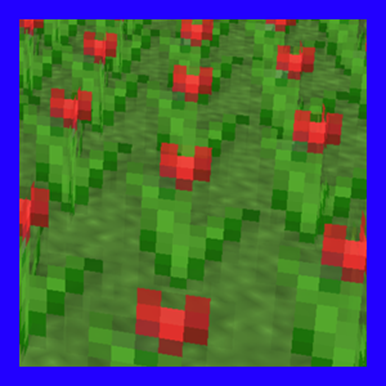
\includegraphics[width=\textwidth]{my_folder/images//oit_flower}
					\caption{Изображение полученное алгоритмом OIT.\linebreak Время построения кадра: 6.2ms}
					\label{fig:oit_flower}
				\end{subfigure}
				\begin{subfigure}[b]{0.3\textwidth}
					\centering
					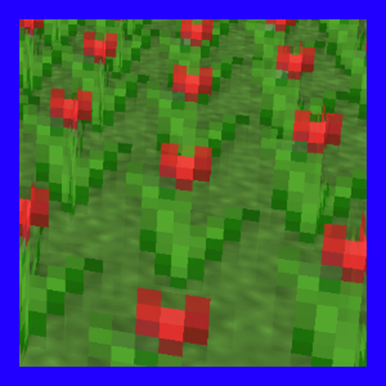
\includegraphics[width=\textwidth]{my_folder/images//hybrid_flower}
					\caption{Изображение полученное алгоритмом Hybrid OIT.\linebreak Время построения кадра: 2.1ms}
					\label{fig:hybrid_flower}
				\end{subfigure}			
				\begin{subfigure}[b]{0.3\textwidth}
					\centering
					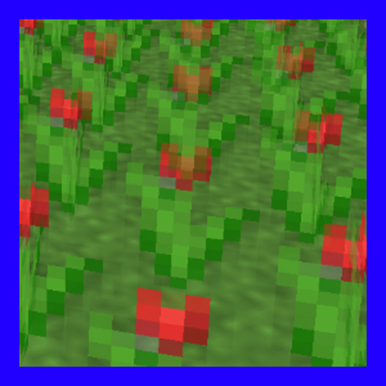
\includegraphics[width=\textwidth]{my_folder/images//wboit_flower}
					\caption{Изображение полученное алгоритмом WBOIT.\linebreak Время построения кадра: 1.9ms}
					\label{fig:wboit_flower}
				\end{subfigure}
			\captionsetup{justification=centering} %центрировать
			\caption{Сравнение работы алгоритмов OIT, WBOIT и Hybrid OIT}\label{fig:oit_vs_wboit_vs_hybrid} 
		\end{figure}